\documentclass[10pt]{article}
\usepackage[polish]{babel}
\usepackage[utf8]{inputenc}
\usepackage[T1]{fontenc}
\usepackage{graphicx}
\usepackage[export]{adjustbox}
\graphicspath{ {./images/} }
\usepackage{amsmath}
\usepackage{amsfonts}
\usepackage{amssymb}
\usepackage[version=4]{mhchem}
\usepackage{stmaryrd}
\usepackage{hyperref}
\hypersetup{colorlinks=true, linkcolor=blue, filecolor=magenta, urlcolor=cyan,}
\urlstyle{same}

\title{GIMNAZJUM }

\author{}
\date{}


\begin{document}
\maketitle
\begin{enumerate}
  \item Ile wynosi pole zacieniowanego obszaru?
  \item Dwaj mężczyźni i dwaj chłopcy zamierzają przepłynąć rzekę, używając do tego celu małej łódki, mogącej pomieścić\\
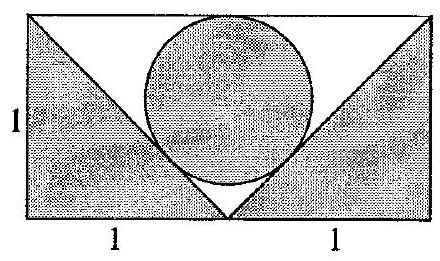
\includegraphics[max width=\textwidth, center]{2024_11_21_78948defe3ef45fddd28g-1(1)}\\
albo jednego mężczyznę, albo dwóch chłopców. Ile co najmniej razy należy przepłynąć rzekę, aby przetransportować całą czwórkę na jej drugą stronę?
  \item Wujek Antoni złowił pewną liczbę ryb. Trzy największe spośród nich dał cioci Halinie, w wyniku czego waga złowionych ryb zmalała o 35\%. Następnie trzy najmniejsze ryby dał sąsiadowi, zmniejszając wagę pozostałych ryb \(\circ \frac{5}{13}\). Ile ryb złowił wujek Antoni?
\end{enumerate}

\section*{LICEUM}
\begin{enumerate}
  \item Ile jest dodatnich liczb całkowitych, których największy dzielnik właściwy (tzn. dzielnik różny od 1 i od danej liczby) wynosi 91?
  \item Jeżeli ABCD jest prostokątem, k - okręgiem o środku w punkcie A, przechodzącym przez C, to jaka jest długość cięciwy EF?
  \item Przekątne AD, BE, CF sześciokąta wypukłego ABCDEF przecinają się w jednym punkcie T, jak zaznaczono na rysunku. Liczby umieszczone na tym rysunku oznaczają pola odpowiednich trójkątów. Ile wynosi pole trójkąta FAT?\\
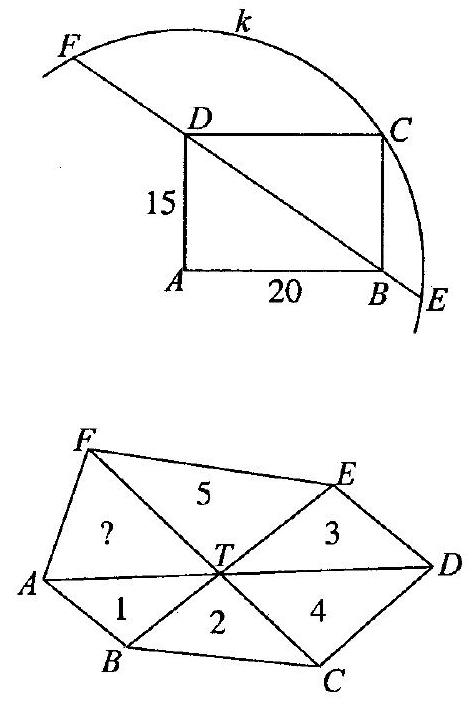
\includegraphics[max width=\textwidth, center]{2024_11_21_78948defe3ef45fddd28g-1}
\end{enumerate}

Rozwiazzania należy oddać do piatku 26 lutego do godziny 10.35 koordynatorowi konkursu panu Jarosławowi Szczepaniakowi lub swojemu nauczycielowi matematyki lub przestać na adres \href{mailto:jareksz@interia.pl}{jareksz@interia.pl} do piątku 26 lutego do pótnocy.


\end{document}